\chapter{Phi to the Fourth Theory}

\section{Leading order calculation of $Z[J]$}

\begin{align}
  Z_0[J] &= e^{-\frac{1}{2}\int \dn{4}{x}\dn{4}{x'}J(x)\Delta(x-x')J(x')} \notag\\
  &= e^{-\frac{1}{2}\vev{J\Delta J}},
\end{align}
and
\begin{align}
  Z[J] &= \No\[1+\(-\imath\frac{\lambda}{4!}\)\int \dn{4}{z}\(\frac{1}{\imath}\frac{\delta}{\delta J(z)}\)^4\]Z_0[J] \notag\\
  &= \No\[1 - \imath\frac{\lambda}{4!}\int \dn{4}{z}\(\frac{\delta}{\delta J_z}\)^4\]Z_0[J].
\end{align}
Then, the derivatives acting on $Z_0[J]$ yield,
\begin{align}
  \frac{\delta}{\delta J_z}Z_0[J] &= -\vev{\Delta J}_z Z_0[J],\\
  \frac{\delta^2}{\delta J_z^2}Z_0[J] &= \[- \Delta_{zz} + \vev{\Delta J}_z^2 \] Z_0[J],\\
  \frac{\delta^3}{\delta J_z^3}Z_0[J] &= \[ 3 \Delta_{zz}\vev{\Delta J}_z - \vev{\Delta J}_z^3 \] Z_0[J],\\
  \frac{\delta^4}{\delta J_z^4}Z_0[J] &= \[ 3 \Delta_{zz}{}^2 - 6 \Delta_{zz}\vev{\Delta J}_z^2 + \vev{\Delta J}_z^4 \] Z_0[J].
\end{align}
Therefore,
\begin{align}
  Z[J] &= \No\Bigg[Z_0[J] -\frac{\imath\lambda}{8}\int\dn{4}{z}\Delta_{zz}{}^2Z_0[J] + \frac{\imath\lambda}{4}\int\dn{4}{z}\Delta_{zz}\vev{\Delta J}_z^2Z_0[J]\notag\\
  &\qquad - \frac{\imath\lambda}{24}\int\dn{4}{z}\vev{\Delta J}_z^4 Z_0[J]\Bigg].\label{GenFun:firstorder}
\end{align}
These expression can be represented graphically, by using Feynman's diagrams, as follows
\begin{align}
  Z[J] = \No\[ 1
  - \frac{\imath\lambda}{8}\;
  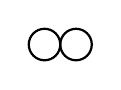
\begin{tikzpicture}[thick] %,baseline=(current bounding box)]
    \draw (2mm,0) circle (2mm);
    \draw (-2mm,0) circle (2mm);
  \end{tikzpicture}
  + \frac{\imath\lambda}{4}\;
  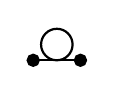
\begin{tikzpicture}[thick]%,baseline=(current bounding box)]
    \draw plot[polar comb,mark=*] coordinates { (0:3mm) (180:3mm) };
    \draw (0,2mm) circle (2mm);
  \end{tikzpicture}
  - \frac{\imath\lambda}{24}\;
  
\begin{tikzpicture}[thick] %,baseline=(current bounding box)]
    \draw plot[polar comb,mark=*] coordinates { (45:3mm) (135:3mm) (-135:3mm) (-45:3mm) };    
  \end{tikzpicture}
  \] Z_0[J].
\end{align}

In order to find the normalisation factor, $\No$, one ask for
\begin{align}
  Z[J=0]=1,
\end{align}
then,
\begin{align}
  \No = \frac{1}{1 - \frac{\imath\lambda}{8}\int\dn{4}{z}\Delta_{zz}{}^2} \simeq 1 + \frac{\imath\lambda}{8}\int\dn{4}{z}\Delta_{zz}{}^2+\Or(\lambda^2),
\end{align}
which can be represented graphically by
\begin{align}
  \No = \frac{1}{1 - \frac{\imath\lambda}{8}\;
  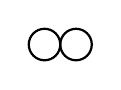
\begin{tikzpicture}[thick] %,baseline=(current bounding box.center)]
    \draw (2mm,0) circle (2mm);
    \draw (-2mm,0) circle (2mm);
  \end{tikzpicture}
  }
  = 1 + \frac{\imath\lambda}{8}\;
  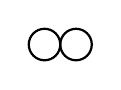
\begin{tikzpicture}[thick] %,baseline=(current bounding box.center)]
    \draw (2mm,0) circle (2mm);
    \draw (-2mm,0) circle (2mm);
  \end{tikzpicture}
  +\Or(\lambda^2).
\end{align}
Note that the normalisation factor is composed by ``vacuum bubbles'', and order by order this cancel the ``vacuum bubbles'' contribution to the calculation of the generating functional,
\begin{align}
  Z[J] &= \frac{1}{1 - \frac{\imath\lambda}{8}\;
  \begin{tikzpicture}[thick,baseline=-\the\dimexpr\fontdimen22\textfont2\relax] %,baseline=(current bounding box.center)]
    \draw (2mm,0) circle (2mm);
    \draw (-2mm,0) circle (2mm);
  \end{tikzpicture}
  }\[ 1
  - \frac{\imath\lambda}{8}\;
  \begin{tikzpicture}[thick,baseline=-\the\dimexpr\fontdimen22\textfont2\relax] %,baseline=(current bounding box)]
    \draw (2mm,0) circle (2mm);
    \draw (-2mm,0) circle (2mm);
  \end{tikzpicture}
  + \frac{\imath\lambda}{4}\;
  \begin{tikzpicture}[thick,baseline=-\the\dimexpr\fontdimen22\textfont2\relax]%,baseline=(current bounding box)]
    \draw plot[polar comb,mark=*] coordinates { (0:3mm) (180:3mm) };
    \draw (0,2mm) circle (2mm);
  \end{tikzpicture}
  - \frac{\imath\lambda}{24}\;
  \begin{tikzpicture}[thick,baseline=-\the\dimexpr\fontdimen22\textfont2\relax] %,baseline=(current bounding box)]
    \draw plot[polar comb,mark=*] coordinates { (45:3mm) (135:3mm) (-135:3mm) (-45:3mm) };    
  \end{tikzpicture}
  \] Z_0[J] \notag\\
  &= \[ 1
  + \frac{\imath\lambda}{4}\;
  \begin{tikzpicture}[thick,baseline=-\the\dimexpr\fontdimen22\textfont2\relax]%%,baseline=(current bounding box)]
    \draw plot[polar comb,mark=*] coordinates { (0:3mm) (180:3mm) };
    \draw (0,2mm) circle (2mm);
  \end{tikzpicture}
  - \frac{\imath\lambda}{24}\;
  \begin{tikzpicture}[thick,baseline=-\the\dimexpr\fontdimen22\textfont2\relax] %,baseline=(current bounding box)]
    \draw plot[polar comb,mark=*] coordinates { (45:3mm) (135:3mm) (-135:3mm) (-45:3mm) };    
  \end{tikzpicture}
  \] Z_0[J] \label{GenFun:FOgraph} \\
  &= \Bigg[1  + \frac{\imath\lambda}{4}\int\dn{4}{z}\Delta_{zz}\vev{\Delta J}_z^2 - \frac{\imath\lambda}{24}\int\dn{4}{z}\vev{\Delta J}_z^4\Bigg] Z_0[J].\label{GenFun:FO}
\end{align}

\section{Two-point Green's Function to First Order}

From the generating function, $Z[J]$, the $n$-point Green's function can be obtained through the relation
\begin{align}
  G^{(n)}(x_1,\cdots,x_n) = \left.\frac{1}{\imath^n}\frac{\delta^n Z[J]}{\delta J_1\cdots \delta J_n}\right|_{J=0}.
\end{align}

Therefore, from Eq.~\eqref{GenFun:FO} one obtains
\begin{align}
  G^{(2)}(x_1,x_2) &= -\left.\frac{\delta^2}{\delta J_1 \delta J_2}\[ 1 + \frac{\imath\lambda}{4}\int\dn{4}{z}\Delta_{zz}\vev{\Delta J}_z^2 - \frac{\imath\lambda}{24}\int\dn{4}{z}\vev{\Delta J}_z^4\] Z_0[J]\right|_{J=0} \notag\\
  &= -\[ -\Delta_{12} + \frac{\imath\lambda}{2}\int\dn{4}{z}\Delta_{zz}{\Delta }_{z1}{\Delta }_{z2}\] \notag\\
  &= 
  \begin{tikzpicture}[thick,baseline=-\the\dimexpr\fontdimen22\textfont2\relax] %,baseline=(current bounding box.center),scale=2]
    \draw (-3mm,0)   -- (3mm,0);
  \end{tikzpicture}
  - \frac{\imath\lambda}{2}\;
  \begin{tikzpicture}[thick,scale=2,baseline=-\the\dimexpr\fontdimen22\textfont2\relax] %]
    \draw (-3mm,0)  -- (3mm,0);
    \draw (0,2mm) circle (2mm);
  \end{tikzpicture}
\end{align}

\section{Four-point Green's Function to First Order}

From Eq.~\eqref{GenFun:FO}, and
\begin{align}
  G^{(4)}(x_1,\cdots,x_4) &= \left.\frac{1}{\imath^4}\frac{\delta^4 Z[J]}{\delta J_1\cdots \delta J_4}\right|_{J=0}\notag\\
  &= \left.\frac{\delta^4 Z[J]}{\delta J_1\cdots \delta J_4}\right|_{J=0},
\end{align}
it follows that
\begin{align}
  \fder{Z[J]}{J_1} &= \Bigg[
    \vev{\Delta J}_1
    + \frac{\imath\lambda}{2}\Delta_{zz}\Delta_{z1}\vev{\Delta J}_z
    - \frac{\imath\lambda}{4} \Delta_{zz} \vev{\Delta J}_z^2 \vdj{1} \notag\\
    & \qquad - \frac{\imath\lambda}{3!}\Delta_{z1}\vdj{z}^3
    + \Or(J^4)\Bigg]Z_0[J] \\
  \frac{\delta^2Z[J]}{\delta J_1\delta J_2} &= \Bigg[
    - \Delta_{12}
    + \frac{\imath\lambda}{2} \Delta_{zz} \Bigg(
    \Delta_{z1}\Delta_{z2}
    + \Delta_{z1}\vdj{z}\vdj{2}
    + \Delta_{z2}\vdj{z}\vdj{1}  \notag\\
    & \qquad \qquad
    + \Delta_{z1}\Delta_{z2}\vdj{z}^2\Bigg)
    -\frac{\imath\lambda}{4} \Delta_{zz}\Delta_{12}\vdj{z}^2
    +\Or(J^3)
    \Bigg] Z_0[J]\\
  \fdern[3]{Z[J]}{J_1}{J_3} &= \Bigg[
    \Delta_{12}\vdj{3}
    + \Delta_{13} \vdj{2}
    + \Delta_{23}\vdj{1} \notag\\
    & \qquad - \frac{\imath\lambda}{2} \Delta_{zz} \Bigg(
    \Delta_{z1}\Delta_{z2}\vdj{3}
    + \Delta_{z1}\Delta_{z3}\vdj{2}
    + \Delta_{z2}\Delta_{z3}\vdj{1} \notag\\
    & \qquad \qquad + \Delta_{z1}\Delta_{23}\vdj{z}
    + \Delta_{z2}\Delta_{13}\vdj{z}
    + \Delta_{z3}\Delta_{12}\vdj{z} \Bigg) \notag\\
    & \qquad - \imath\lambda \Delta_{z1}\Delta_{z2}\Delta_{z3}\vdj{z}
    +\Or(J^2) \Bigg]Z_0[J] \\
  \fdern[4]{Z[J]}{J_1}{J_4} &= \Bigg[
    \Delta_{12}\Delta_{34}
    + \Delta_{13}\Delta_{24}
    + \Delta_{14}\Delta_{23} \notag\\
    & \qquad - \frac{\imath\lambda}{2} \Delta_{zz} \Bigg(
    \Delta_{z1}\Delta_{z2}\Delta_{34}
    + \Delta_{z1}\Delta_{z3}\Delta_{24}
    + \Delta_{z1}\Delta_{z4}\Delta_{23} \notag\\
    & \qquad \qquad
    + \Delta_{z2}\Delta_{z3}\Delta_{14}
    + \Delta_{z2}\Delta_{z4}\Delta_{13}
    + \Delta_{z3}\Delta_{z4}\Delta_{12} \Bigg) \notag\\
    & \qquad
    - \imath\lambda \Delta_{z1}\Delta_{z2}\Delta_{z3}\Delta_{z4}
    \Bigg]Z_0[J].
\end{align}
Therefore,
\begin{align}
  G^{(4)}(x_1,\cdots,x_4) &=
      \Delta_{12}\Delta_{34}
    + \Delta_{13}\Delta_{24}
    + \Delta_{14}\Delta_{23} \notag\\
    & \quad - \frac{\imath\lambda}{2} \Delta_{zz} \Bigg(
    \Delta_{z1}\Delta_{z2}\Delta_{34}
    + \Delta_{z1}\Delta_{z3}\Delta_{24}
    + \Delta_{z1}\Delta_{z4}\Delta_{23} \notag\\
    & \qquad \qquad
    + \Delta_{z2}\Delta_{z3}\Delta_{14}
    + \Delta_{z2}\Delta_{z4}\Delta_{13}
    + \Delta_{z3}\Delta_{z4}\Delta_{12} \Bigg) \notag\\
    & \quad
    - \imath\lambda \Delta_{z1}\Delta_{z2}\Delta_{z3}\Delta_{z4}
\end{align}

Graphically,
\begin{align}
  G^{(4)}(x_1,\cdots,x_4) &=
  \mbox{
    \begin{tikzpicture}[thick,baseline=-\the\dimexpr\fontdimen22\textfont2\relax]%baseline=(current bounding box.center)]
      \pgfmathsetmacro{\d}{.3}
      \draw (-\d,\d) -- (\d,\d);
      \draw (-\d,-\d) -- (\d,-\d);
    \end{tikzpicture}
  }
  +
  \mbox{
    \begin{tikzpicture}[thick,baseline=-\the\dimexpr\fontdimen22\textfont2\relax]%baseline=(current bounding box.center)]
      \pgfmathsetmacro{\d}{.3}
      \draw (-\d,\d) -- (-\d,-\d);
      \draw (\d,\d) -- (\d,-\d);
    \end{tikzpicture}
  }
  +
  \mbox{
    \begin{tikzpicture}[thick,baseline=-\the\dimexpr\fontdimen22\textfont2\relax]%baseline=(current bounding box.center)]
      \pgfmathsetmacro{\d}{.3}
      \draw (-\d,\d) -- (\d,-\d);
      \fill[white] (0,0) circle (1.5pt);
      \draw (-\d,-\d) -- (\d,\d);
    \end{tikzpicture}
  }
  \notag \\
  & \quad
  - \frac{\imath\lambda}{2} \Bigg(
  \begin{tikzpicture}[thick,baseline=-\the\dimexpr\fontdimen22\textfont2\relax]%baseline=(current bounding box.center)]
    \pgfmathsetmacro{\d}{.3}
    \draw (-\d,\d) -- (\d,\d);
    \draw (0,{\d cm -1mm}) circle (1mm); 
    \draw (-\d,-\d) -- (\d,-\d);
  \end{tikzpicture}
  +
  \begin{tikzpicture}[thick,baseline=-\the\dimexpr\fontdimen22\textfont2\relax]%baseline=(current bounding box.center)]
    \pgfmathsetmacro{\d}{.3}
    \draw (-\d,\d) -- (\d,\d);
    \draw (-\d,-\d) -- (\d,-\d);
    \draw (0,{-\d cm + 1mm}) circle (1mm);
  \end{tikzpicture}
  +
  \begin{tikzpicture}[thick,baseline=-\the\dimexpr\fontdimen22\textfont2\relax]%baseline=(current bounding box.center)]
    \pgfmathsetmacro{\d}{.3}
    \draw (-\d,\d) -- (-\d,-\d);
    \draw ({-\d cm + 1mm},0) circle (1mm);
    \draw (\d,\d) -- (\d,-\d);
  \end{tikzpicture}
  +
  \begin{tikzpicture}[thick,baseline=-\the\dimexpr\fontdimen22\textfont2\relax]%baseline=(current bounding box.center)]
    \pgfmathsetmacro{\d}{.3}
    \draw (-\d,\d) -- (-\d,-\d);
    \draw (\d,\d) -- (\d,-\d);
    \draw ({\d cm - 1mm},0) circle (1mm);
  \end{tikzpicture}
  +
  \begin{tikzpicture}[thick,baseline=-\the\dimexpr\fontdimen22\textfont2\relax]%baseline=(current bounding box.center)]
    \pgfmathsetmacro{\d}{.3}
    \draw (-\d,\d) -- (\d,-\d);
    \draw ({-\d cm + 1.914mm},{\d cm - 0.5mm}) circle (1mm);
    \fill[white] (0,0) circle (1.5pt);
    \draw (-\d,-\d) -- (\d,\d);
  \end{tikzpicture}
  +
  \begin{tikzpicture}[thick,baseline=-\the\dimexpr\fontdimen22\textfont2\relax]%baseline=(current bounding box.center)]
    \pgfmathsetmacro{\d}{.3}
    \draw (-\d,\d) -- (\d,-\d);
    \fill[white] (0,0) circle (1.5pt);
    \draw (-\d,-\d) -- (\d,\d);
    \draw ({-\d cm + 1.914mm},{-\d cm + 0.5mm}) circle (1mm);
  \end{tikzpicture}
  \Bigg)
  \notag\\
  & \quad
  - \imath\lambda
  \mbox{
    \begin{tikzpicture}[thick,baseline=-\the\dimexpr\fontdimen22\textfont2\relax]
      \coordinate (V) at (0,0);
      \pgfmathsetmacro{\d}{.3}
      \draw (V) -- (\d,\d);
      \draw (V) -- (-\d,\d);
      \draw (V) -- (-\d,-\d);
      \draw (V) -- (\d,-\d);
    \end{tikzpicture}
  }
\end{align}

\chapter{Grassmann integration}

\begin{align}
  \ket{\psi} = e^{b^{\dag}\psi}\ket{0},\qquad \bra{\bps}=\bra{0}e^{\bps b}.\label{FermCoher}
\end{align}
Then,
\begin{align}
  \int \de{\bps}\de{\psi}\;e^{-\bps\psi}\ket{\psi}\bra{\bps}
  &= \int \de{\bps}\de{\psi}\;\({1 - \bps\psi}\)\ket{\psi}\bra{\bps} \notag\\
  &= \int \de{\bps}\de{\psi}\;\[{1 - \bps\psi}\]e^{b^{\dag}\psi}\ket{0}\bra{0}e^{\bps b} \notag\\
  &= \int \de{\bps}\de{\psi}\;\[{1 - \bps\psi}\]\(\ket{0} - \psi\ket{1}\)\(\bra{0} - \bra{1}\bps\) \notag\\
  &= \int \de{\bps}\de{\psi}\;\[\( \psi\ket{1}\bra{1}\bps\) - \(\bps\psi\ket{0}\bra{0}\)\] \notag\\
  &= \ket{0}\bra{0} + \ket{1}\bra{1} \notag\\
  &= \mathds{1}
\end{align}

From  Eq.~\eqref{FermCoher}, one obtain
\begin{align}
  b\ket{\psi} &= b\(e^{b^{\dag}\psi}\ket{0}\)\notag\\
  &= b \(\ket{0} - \psi\ket{1}\) \notag\\
  &= \psi b \,b^\dag \ket{0} \notag\\
  &= \psi \( 1- b^\dag b\) \ket{0} \notag\\
  &= \psi\ket{0} \notag\\
  &= \psi\ket{\psi},
\end{align}
and
\begin{align}
  b^{\dag}\ket{\psi} &= b^{\dag}\(e^{b^{\dag}\psi}\ket{0}\)\notag\\
  &= b^{\dag} \(\ket{0} - \psi\ket{1}\) \notag\\
  &= b^{\dag} \ket{0} \notag\\
  &= -\fder{}{\psi} \ket{\psi}.
\end{align}


The Gaussian integration of Grassman variables,
\begin{align}
  \int \de{\bps} \de{\psi}\; e^{\bet\psi+\bps\eta+\delta\bps\psi} 
  &= \int \de{\bps} \de{\psi}\;e^{\bet\psi+\bps\eta+\bps\delta\psi} \notag\\
  &= \int \de{\bps} \de{\psi}\;e^{\(\bps + \bet \delta^{-1}\)\delta\(\delta^{-1}\eta +\psi\)}e^{-\bet\delta^{-1}\eta} \notag\\
  &= e^{-\bet\delta^{-1}\eta} \int \de{\bps'} \de{\psi'}\;e^{\bps' \delta \psi'} \notag\\
  &= -\delta\,e^{-\bet\delta^{-1}\eta}.
\end{align}




\chapter{Gauge Theories}

In four dimensions, one might define the dual of the field strength, ${}^*F_{\mu\nu}^a$, by
\begin{align}
  {}^*F_{\mu\nu}^a = \frac{1}{2}\epsilon_{\mu\nu\lambda\rho} F^{a\,\lambda\rho}.
\end{align}
The construction ${}^*F_{\mu\nu}^a F^{a\,\mu\nu}$ is Lorentz and gauge invariant and can be added to the Lagrangian.

However, 
\begin{align}
  {}^*F_{\mu\nu}^a F^{a\,\mu\nu}
  &= \frac{1}{2}\epsilon_{\mu\nu\lambda\rho} F^{a\,\lambda\rho}F^{a\,\mu\nu}\notag\\
  &= \frac{1}{2}\epsilon_{\mu\nu\lambda\rho} \(\pau{\lambda}A^{a\,\rho}-\pau{\rho}A^{a\,\lambda}\)F^{a\,\mu\nu}\notag\\
  &= \frac{1}{2}\epsilon_{\mu\nu\lambda\rho} \(\nabla^{\lambda}A^{a\,\rho}-\nabla^{\rho}A^{a\,\lambda}\)F^{a\,\mu\nu}\notag\\
  &= \epsilon_{\mu\nu\lambda\rho} \nabla^{\lambda}A^{a\,\rho}F^{a\,\mu\nu}\notag\\
  &= \pau{\lambda}\(\epsilon_{\mu\nu\lambda\rho} A^{a\,\rho}F^{a\,\mu\nu}\) - \epsilon_{\mu\nu\lambda\rho} A^{a\,\rho}\(\nabla^{\lambda}F^{a\,\mu\nu}\), \label{ThetaTerm}
\end{align}
the last term vanishes due to the Bianchi identity, and the remaining one is a total derivative which does not contribute to the equations of motion. 

Equation~\eqref{ThetaTerm} can be represented as the derivative of a current, $K^\mu$, with
\begin{align}
  K^\mu = \epsilon_{\mu\nu\lambda\rho} A^{a\,\rho}F^{a\,\mu\nu}.
\end{align}

\section{Chern-Simons action}

In three-dimensional spacetime, there is another possibility of constructing a gauge invariant action, called the Chern-Simons action,
\begin{align}
  S = \int\dn{3}{x}\epsilon^{\mu\nu\lambda}\[A^a_\mu\pa{\nu}A^a_\lambda + \frac{1}{3}f^{abc}A^a_\mu A^b_\nu A^c_\lambda\] + \int\dn{3}{x} A^a_\mu J^{a\,\mu}.
\end{align}

The equations of motion for this action are given by the Euler-Lagrange equations,
\begin{align}
  \pa{\alpha}\(\fder{\Lag}{\pa{\alpha}A^m_{\beta}}\) - \fder{\Lag}{A^m_{\beta}} =0.
\end{align}

Since,
\begin{align}
  \pa{\alpha}\(\fder{\Lag}{\pa{\alpha}A^m_\beta}\) &= \epsilon^{\mu\alpha\beta}\pa{\alpha}A^m_\mu, \\
  \fder{\Lag}{A^m_\beta} &= \epsilon^{\beta\nu\lambda}\[\pa{\nu}A^m_\lambda + \frac{1}{2}f^{mbc} A^b_\nu A^c_\lambda\] + J^m_\beta,
\end{align}
then, the equations of motion are
\begin{align}
  - \epsilon^{\beta\nu\lambda}\[\pa{\nu}A^m_\lambda - \pa{\lambda}A^m_\nu + \frac{1}{2}f^{mbc} A^b_\nu A^c_\lambda\] = J^m_\beta
\end{align}
or
\begin{align}
  - \epsilon^{\beta\nu\lambda} F^m_{\nu\lambda} = J^m_\beta.
\end{align}
